\documentclass[twocolumn,10pt]{jarticle}
\setlength{\columnsep}{3zw}

\usepackage[dvipdfmx]{graphicx}

\graphicspath{{./image/}}

\title{実験計画}

\author{奥屋 直己}

\usepackage[height=26cm,width=16cm]{geometry}

\begin{document}

\maketitle

\section{目的}
音楽の演奏において、テンポを一定に保ち続けることは最も重要なことの一つである。しかし、演奏者の意図にかかわらずにテンポ変化が生じることがあり、そのような場合の多くは、テンポが加速する方向に変化する。このような意図しないテンポ変化は、演奏者の間で「走る」という表現で共有され、だれもがよく経験することである。このテンポ加速現象は古くから検討されてきたが、従来の実験の多くが一定時間間隔のタッピング課題を対称としており、リズムや強弱といった実際の音楽演奏に含まれるリズムパタンの要素を考慮していない(2.永島 亮誠, 阪口 豊)。また、同一のリズムパタンであっても、振り上げる腕の位置やタッピングの強さというの要素も考慮すべきである。本実験ではリズムやアクセントパタンを伴うタッピングの同期課題と、タッピングする指の位置、タッピングの強さ、これらの要素がテンポ維持特性に与える影響を実験的に検討する。

\section{実験方法}
\subsection{被験者}
本実験には10名(男性○、女性○)の被験者が参加した。楽器演奏経験の乏しい被験者では安定したリズムパタンの再生が困難である場合が多いため、本実験の被験者には何らかの楽器演奏経験がある被験者のみを対象に行った。被験者には謝礼として、図書カード1000円分を手渡した。
\subsection{課題}
本実験には、従来の研究と同様に同期・継続課題を用いる。従来の研究と異なる点では、テンポだけでなくリズムを含めて目標音と同期してタッピングし、また、それを継続する点である。本実験では、同期区間を32拍分(4分の4拍子で8小節)、継続区間を320拍分(4分の4拍子で80小節)とした。

本研究では、Collyer,et al. の報告[1]においてテンポ変化が生じにくかった120 bpmを目標テンポに設定して目標リズム音を作成した。

\subsection{装置}
被験者のタッピング動作の記録には、Arduinoに圧力センサ、赤外線距離センサを組み合わせたスイッチも用いる。被験者はこのスイッチを人差し指でタッピングすることにより課題を遂行する。Arduinoと計測用PCをUSBケーブルを介して接続され、圧力センサと距離センサの数値は、時間とともに随時テキストファイルに書き込む。また、目標とするリズムパタンの生成は、Garageband上の打楽器音にて作成した、mp3音源を使用した。目標リズム音は、Arduinoの計測開始と同期し、同期区間8小節のみ再生した。再生にはスピーカー(なんかのやつ)を使用し、被験者ごとに快適な音量に調節し、提示した。

\subsection{条件}
本実験では、タッピング間隔が一定である統制条件と、他合計8種類のリズムおよびアクセントパタンでタッピングを行う条件を設ける。条件aは統制条件、c-dは(2.永島 亮誠, 阪口 豊)の研究で加速が見られたパタン、e-fは同実験で減速が見られたパタン、g-hは2小節を1つとしたリズムパタンである。
\subsubsection{手続き}
各実験での課題になれるために、同期区間8小節、継続区間8小節の練習課題を課す。被験者がリズムパタンを理解したことを確認した後、被験者がリズムパタンを理解したことを確認した後、同期区間 32拍分、継続区間 320拍分の本試験を行う。
\begin{center}
	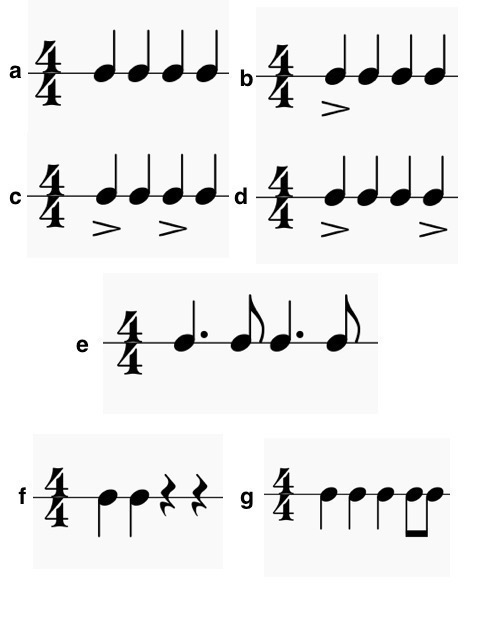
\includegraphics[width=6cm]{patna_g.jpeg}
\end{center}	
\begin{center}
	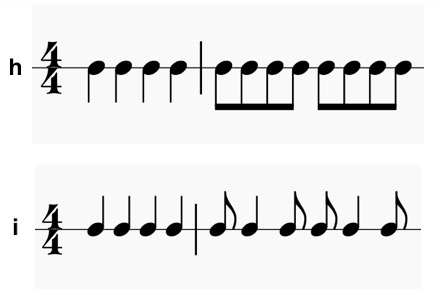
\includegraphics[width=6cm]{patnh_i.jpeg}
\end{center}	






\section{文献}
\begin{enumerate}
  \item Collyer, C., Broadbent, H., \& Church, R.(1992).Categorical time production: Evidence for discrete timing in motor control. {\it Preception \& Psychonomic bulletin \& Psychophysics, 51(2),134-144.}
  \item 永島 亮誠, 阪口 豊. (2018) "リズムパタンや強弱の時間パタンがテンポ維持特性に与える影響"
\end{enumerate}
\end{document}